% Snowflake Data Engineering — Chapter 12 | original manuscript draft
% Author: Arman Golbidi | Editorial snapshot: 22 October 2026
% Compile: xelatex -interaction=nonstopmode -halt-on-error Snowflake_Data_Engineering_Chapter_11.tex
% Trim: 178 x 254 mm; margins inside 23 mm / outside 17 mm / top-bottom 19 mm.
% Body: 10.75 pt / 13.65 pt leading = 1.27 line-height ratio; code: 8.75 pt.
\documentclass[11pt,twoside]{article}
\usepackage[paperwidth=178mm,paperheight=254mm,inner=23mm,outer=17mm,top=19mm,bottom=19mm,headheight=5mm,headsep=4mm,footskip=9mm]{geometry}
\usepackage{fontspec}
\setmainfont{LibertinusSerif-Regular.otf}[BoldFont=LibertinusSerif-Bold.otf,ItalicFont=LibertinusSerif-Italic.otf,BoldItalicFont=LibertinusSerif-BoldItalic.otf]
\setsansfont{LibertinusSans-Regular.otf}[BoldFont=LibertinusSans-Bold.otf,ItalicFont=LibertinusSans-Italic.otf]
\setmonofont{LibertinusMono-Regular.otf}[Scale=0.91]
\usepackage[english]{babel}
\usepackage{microtype}
\usepackage{setspace}
\setstretch{1.0}
\usepackage{titlesec,enumitem,tabularx,array,booktabs,needspace,fancyhdr,lastpage}
\usepackage[most]{tcolorbox}
\usepackage{tikz}
\usetikzlibrary{arrows.meta,positioning,fit,shapes.misc,calc}
\usepackage{listings}
\usepackage{xcolor}
\usepackage{hyperref}
\usepackage{amsmath}
\hypersetup{colorlinks=true,urlcolor=steelblue,linkcolor=steelblue,pdfauthor={Arman Golbidi},pdftitle={Snowflake Data Engineering - Chapter 12: Query Performance and Warehouse Optimization},pdfsubject={English technical book manuscript, twelfth chapter, 178 x 254 mm}}
\definecolor{navy}{HTML}{15334A}
\definecolor{steelblue}{HTML}{17779B}
\definecolor{teal}{HTML}{12888A}
\definecolor{lightblue}{HTML}{ECF5F7}
\definecolor{papergray}{HTML}{F2F5F6}
\definecolor{inkgray}{HTML}{4A5862}
\definecolor{thinrule}{HTML}{CBD7DB}
\AtBeginDocument{\color{navy}\fontsize{10.75}{13.65}\selectfont}
\setlength{\parindent}{0pt}
\emergencystretch=2.5em
\setlength{\parskip}{3.3pt plus 0.7pt minus 0.6pt}
\setlist[itemize]{leftmargin=4mm,itemsep=1pt,topsep=2pt,parsep=0pt}
\setlist[enumerate]{leftmargin=5mm,itemsep=1pt,topsep=2pt}
\titleformat{\section}{\sffamily\bfseries\color{navy}\fontsize{14}{17}\selectfont}{}{0pt}{}
\titlespacing*{\section}{0pt}{8pt}{4pt}
\titleformat{\subsection}{\sffamily\bfseries\color{steelblue}\fontsize{10.8}{13}\selectfont}{}{0pt}{}
\titlespacing*{\subsection}{0pt}{5pt}{1pt}
\newcommand{\topic}[2]{\subsection*{#1\quad #2}}
\newcommand{\repo}[2]{\par\begingroup\fontsize{8.0}{9.6}\selectfont\sffamily\color{inkgray}\textbf{Project reference:} \href{#2}{#1}. \textit{Not independently executed; rights review pending.}\par\endgroup}
\newtcolorbox{insight}[1][]{enhanced,breakable,colback=lightblue,colframe=thinrule,boxrule=.45pt,arc=1.3mm,left=2.8mm,right=2.8mm,top=1.8mm,bottom=1.8mm,before skip=5pt,after skip=5pt,#1}
\newtcolorbox{whitebox}[1][]{enhanced,breakable,colback=papergray,colframe=thinrule,boxrule=.35pt,arc=1mm,left=2.6mm,right=2.6mm,top=1.5mm,bottom=1.5mm,before skip=4pt,after skip=5pt,#1}
\lstdefinestyle{chaptercode}{basicstyle=\ttfamily\fontsize{8.75}{10.7}\selectfont,backgroundcolor=\color{papergray},frame=single,framerule=.35pt,rulecolor=\color{thinrule},breaklines=true,columns=fullflexible,keepspaces=true,showstringspaces=false,aboveskip=5pt,belowskip=5pt,xleftmargin=2mm,xrightmargin=1mm,framexleftmargin=2mm,framexrightmargin=1mm}
\lstset{style=chaptercode}
\pagestyle{fancy}
\fancyhf{}
\fancyhead[LE]{\sffamily\fontsize{7.6}{9}\selectfont\color{inkgray}\textsc{Snowflake Data Engineering}}
\fancyhead[RO]{\sffamily\fontsize{7.6}{9}\selectfont\color{inkgray}\textsc{12 / Performance \& Cost}}
\fancyfoot[LE,RO]{\sffamily\bfseries\fontsize{8.2}{9}\selectfont\color{steelblue}\thepage}
\fancyfoot[LO,RE]{\sffamily\fontsize{7.6}{9}\selectfont\color{inkgray}Arman Golbidi \quad | \quad Chapter 12}
\renewcommand{\headrulewidth}{0.35pt}
\renewcommand{\footrulewidth}{0pt}
\setcounter{page}{209}
\raggedbottom

\begin{document}
% PAGE 209
{\sffamily\bfseries\fontsize{9}{11}\selectfont\color{steelblue} CHAPTER 12 \hfill PERFORMANCE / EVIDENCE / CREDITS}\par\vspace{3mm}
{\sffamily\bfseries\fontsize{20.0}{23}\selectfont\color{navy} Query Performance and\\Warehouse Optimization}\par\vspace{2mm}
{\sffamily\fontsize{11}{14}\selectfont\color{steelblue} Make the query correct; diagnose the bottleneck; then spend deliberately}\par\vspace{3mm}
\begin{insight}\textbf{The tempting fix is to double the warehouse.}\par
At 08:30 a Power BI report that normally opens promptly starts taking twenty seconds. The data engineer increases the Snowflake warehouse size. The next screen loads quickly, but the team cannot say whether resizing helped: the first request resumed a suspended warehouse, the second benefited from cache, and the underlying SQL unexpectedly duplicates generation rows after joining a many-to-many lookup. Credits rise while the KPI remains wrong. A faster answer is not an improved system when it answers the wrong question.
\end{insight}
This chapter provides an investigation method for the \emph{Finland Energy Analytics} platform. Building on Chapters~2, 4 and 11, it connects the semantics of a query with evidence from Query History, execution operators, micro-partition pruning, queuing, memory pressure and measured cost. Optimisation is presented as an experiment, not as a collection of magic switches.
\begin{whitebox}\textbf{Learning outcomes}\par
You will: (1) formulate falsifiable tuning hypotheses; (2) compare the same correct result before and after a change; (3) interpret Query Profile and history fields; (4) decide whether pruning, warehouse sizing, clustering, caches, query acceleration or search optimisation addresses the observed bottleneck; (5) report latency and credits honestly; and (6) explain why a result from a six-row teaching fixture cannot predict production performance.\end{whitebox}
\textbf{Prerequisites.} Chapters~2, 4 and 11; SQL \texttt{JOIN}, \texttt{GROUP BY} and time filters; access to a permitted Snowflake test environment for optional cloud runs. Offline lab tests use only synthetic data. Cloud benchmarking may consume credits; agree a budget and use a restricted role.
\begin{center}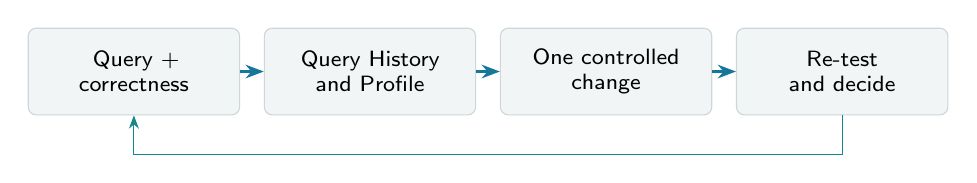
\begin{tikzpicture}[>=Stealth,every node/.style={font=\sffamily\fontsize{7.7}{9}\selectfont},n/.style={draw=thinrule,rounded corners=1mm,fill=papergray,align=center,text width=24.5mm,minimum height=11mm}]
\node[n](a){Query +\\correctness};\node[n,right=3mm of a](b){Query History\\and Profile};\node[n,right=3mm of b](c){One controlled\\change};\node[n,right=3mm of c](d){Re-test\\and decide};
\draw[->,thick,steelblue](a)--(b);\draw[->,thick,steelblue](b)--(c);\draw[->,thick,steelblue](c)--(d);
\draw[->,teal] (d.south) -- ++(0,-5mm) -| (a.south);
\end{tikzpicture}\\{\fontsize{8}{9}\selectfont\color{inkgray}Figure 12.1. Performance work is an evidence loop, not a warehouse-size reflex.}\end{center}
\newpage
% PAGE 210
\section*{12.1\quad A structured performance troubleshooting workflow}
\topic{12.1.1}{Hypotheses and reproducible tests}
Performance work begins with a statement that can be disproved. ``Snowflake is slow'' is not testable. ``The daily energy report scans most partitions because its timestamp predicate cannot exploit the stored range'' is testable: inspect scan ratios, rewrite the filter without changing its meaning, and compare profiles over repeated runs. Record the query text or versioned file, query ID, \texttt{QUERY\_TAG}, warehouse size, account/region, inputs, role, result shape, cache policy and competing workload.

A useful triage sequence is \textbf{scope $\to$ correctness $\to$ wait time $\to$ operators $\to$ candidate change $\to$ repeat}. Distinguish a slow visual from a slow Snowflake statement: report rendering, gateway/network transfer, source SQL compilation, warehouse provisioning and query execution contribute separately to perceived latency. Do not optimise a warehouse on the basis of an uncorrelated stopwatch from the browser.
\begin{lstlisting}[language=SQL,caption={Illustrative session controls: do not change shared warehouses.}]
ALTER SESSION SET QUERY_TAG =
  'book_ch12_energy_benchmark_v1';
ALTER SESSION SET USE_CACHED_RESULT = FALSE;
SELECT CURRENT_ROLE(), CURRENT_WAREHOUSE();
-- Restore at the end of the isolated experiment:
ALTER SESSION UNSET QUERY_TAG;
ALTER SESSION UNSET USE_CACHED_RESULT;
\end{lstlisting}
Disabling persisted query-result reuse does \emph{not} eliminate warehouse-local data caching or other environmental variation. A warm-versus-cold experiment must record warehouse suspension/resume state and cannot assert perfect cache isolation without further controls.
\begin{whitebox}\textbf{Experimental contract}\par
\textbf{Question:} does a half-open timestamp range reduce work compared with an expression around the filtered column? \textbf{Invariant:} identical grouping keys and MWh totals. \textbf{Evidence:} query IDs, scan/partition counts, execution and queuing components, five or more controlled repeats per treatment. \textbf{Decision:} accept only when gains are repeatable and materially exceed operational costs.\end{whitebox}
\repo{P017: sfc-gh-bokon/query\_performance\_deep\_dive}{https://github.com/sfc-gh-bokon/query_performance_deep_dive}
\textbf{Check.} What observation would falsify a theory that pruning is responsible for the delay?
\newpage
% PAGE 211
\topic{12.1.2}{Correctness before speed}
An optimisation may reduce runtime while changing the answer. Consider the running case: six accepted technology observations sum to \textbf{66.000~MWh} for one synthetic UTC interval. If an engineer joins those rows to a technology alias table with two matching aliases per row, a subsequent \texttt{SUM} can silently double production to \textbf{132.000~MWh}. Neither a faster join algorithm nor more compute makes that result acceptable.
\begin{lstlisting}[language=SQL,caption={Confirm the gold grain before joining.}]
SELECT interval_utc, technology, COUNT(*) AS n
FROM BOOK_DEV.CH12_LAB.ENERGY_FACT
GROUP BY interval_utc, technology
HAVING COUNT(*) <> 1;
-- Expected on the provided seven-day fixture: 0 rows.
\end{lstlisting}
For each baseline and proposed rewrite, test \textbf{row count, key uniqueness, null handling, unit consistency and aggregates}. A missing period must not become a zero-valued period unless the business contract explicitly defines imputation. When the source includes revisions, benchmark the deduplicated authoritative state, not all raw deliveries. Compare all result rows (or a deterministic keyed digest) rather than only a total that could conceal offsetting errors.
\begin{insight}\textbf{Two kinds of correctness.}\par
\emph{Semantic correctness} means that generation is measured in MWh, at the intended event-time grain, for the intended geographic and source scope. \emph{Mechanical correctness} means that the query respects uniqueness, grouping and equality of output for a given snapshot. Both must hold.\end{insight}
A practical review pairs each expected result with its computation: \texttt{COUNT(*)=42} and \texttt{SUM(energy\_mwh)=462.000} for the companion's \emph{seven-day expanded synthetic fixture} (six technologies repeated across seven days). These numbers are offline oracle values, not observed Finland generation.
\textbf{Failure diagnosis.} If a rewritten query disagrees, stop timing tests and inspect join multiplicity, time boundaries, \texttt{NULL} behaviour and source versions. \textbf{Check.} Why is matching total MWh alone not enough to prove two queries equivalent?
\newpage
% PAGE 212
\topic{12.1.3}{Isolating the performance bottleneck}
A single elapsed-time number conceals different problems. A statement can wait for a suspended warehouse to resume (provisioning), queue because concurrency exceeds available capacity (overload), compile complex SQL, scan unnecessary partitions, spill intermediate data or transfer a large result across the network. These demand different remedies. Use the \emph{highest-cost observed stage}, not a guessed bottleneck, to choose the next experiment.
\begin{center}\renewcommand{\arraystretch}{1.1}\begin{tabularx}{\linewidth}{@{}p{33mm}XX@{}}\toprule
\textbf{Evidence}&\textbf{Plausible cause}&\textbf{First test}\\\midrule
Provisioning wait&Suspended/cold warehouse&Separate resume from steady-state\\
Overload wait&Concurrent queries&Repeat with controlled concurrency\\
Many partitions scanned&Weak filter pruning&Preserve sargable ranges\\
Remote spill&Large intermediate state&Inspect join/aggregation before resizing\\
Large returned bytes&Excess columns/rows&Return only required fields\\\bottomrule\end{tabularx}\end{center}
Not every indicator is a proof. For example, some workloads legitimately scan nearly all partitions; selective pruning is not meaningful for an unfiltered whole-table aggregation. Similarly, remote spill is usually suspicious but particular services may show nonzero remote-storage metrics for reasons that require profile-level verification. Query compilation can vary independently of scan efficiency.
\begin{center}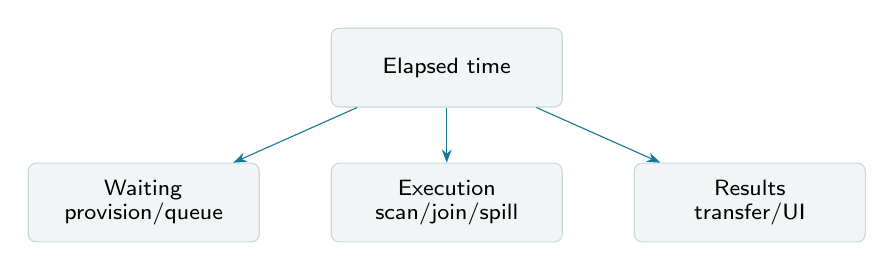
\begin{tikzpicture}[>=Stealth,every node/.style={font=\sffamily\fontsize{7.6}{9}\selectfont},b/.style={draw=thinrule,rounded corners=1mm,fill=papergray,align=center,text width=27mm,minimum height=10mm}]
\node[b](a){Elapsed time};\node[b,below left=7mm and 9mm of a](b){Waiting\\provision/queue};\node[b,below=7mm of a](c){Execution\\scan/join/spill};\node[b,below right=7mm and 9mm of a](d){Results\\transfer/UI};
\draw[->,steelblue](a)--(b);\draw[->,steelblue](a)--(c);\draw[->,steelblue](a)--(d);
\end{tikzpicture}\\{\fontsize{8}{9}\selectfont\color{inkgray}Figure 12.2. One elapsed time may hide three different interventions.}\end{center}
\textbf{Decision rule.} Rewrite an inefficient expression before buying a larger warehouse. Investigate a concurrency bottleneck before changing clustering. Analyse an oversized BI result before enabling a paid acceleration feature. \textbf{Check.} Which metric distinguishes queued overload from a long-running hash aggregation?
\newpage
% PAGE 213
\section*{12.2\quad Query History and Query Profile}
\topic{12.2.1}{Query History metadata}
Snowflake provides recent query details in Snowsight and Information Schema table functions, while \texttt{SNOWFLAKE.ACCOUNT\_USAGE.QUERY\_HISTORY} supports broader historical analysis subject to privileges and reporting latency. Useful fields include query ID and tag, warehouse name/size, status, total elapsed/compilation/execution times, provisioning and overload waits, scanned bytes, scanned/total partitions, result-cache percentages and spill metrics. Field availability and interpretation should be rechecked at publication time.
\begin{lstlisting}[language=SQL,caption={Recent per-user history: permitted users only.}]
SELECT query_id, query_tag, warehouse_name,
       total_elapsed_time, execution_time,
       queued_overload_time, bytes_scanned
FROM TABLE(INFORMATION_SCHEMA.QUERY_HISTORY(
  DATEADD('HOUR', -1, CURRENT_TIMESTAMP()),
  CURRENT_TIMESTAMP(), 100))
WHERE query_tag = 'book_ch12_energy_benchmark_v1'
ORDER BY start_time DESC;
\end{lstlisting}
\emph{Account Usage} can lag behind the most recent execution. For an immediate diagnosis, inspect Snowsight and the appropriate recent-history function; for a retrospective account-wide trend, use a granted monitoring role. Access to observability data is \emph{not} a reason to grant \texttt{ACCOUNTADMIN} to a lab user.
\topic{12.2.2}{Query Profile operators and scans}
Open the saved query ID in Query Profile. Read its execution graph from scans through joins and aggregates to the final result. Compare \emph{actual scanned partitions}, not the verbal presence of a filter. An explicit filter may still scan most table storage when values overlap broadly between micro-partitions; a low scan fraction may already indicate good pruning. Observe rows entering and leaving nodes: a join expanding six rows into twelve can be the root cause of an incorrect total.
\repo{P018: Snowpark Python performance tips}{https://github.com/Snowflake-Labs/sfguide-snowpark-python-top-three-tips-for-optimal-performance}
\textbf{Check.} Why must the time at which Query History becomes visible be recorded separately from the execution time?
\newpage
% PAGE 214
\topic{12.2.3}{Reading spilled data and queuing indicators}
Spill occurs when an operation cannot retain all required intermediate state in available memory. Storage spill to local disk is usually less damaging than remote spill. Sorting, large joins, distinct aggregations and skewed groups are common places to investigate. A larger warehouse may supply more memory, but fixing a cross join or reducing the intermediate working set can be both faster and cheaper. Check the operator-level profile and compare row expansion before resizing.

\textbf{Queuing is not execution.} A query can run in a few hundred milliseconds once scheduled yet wait several seconds behind other requests. Record provisioning wait and overload wait separately from execution; a multi-cluster warehouse primarily addresses concurrent workload throughput where supported, not necessarily the runtime of one serial query. Do not conclude that a clustering key cures queues.
\begin{lstlisting}[language=SQL,caption={Historical diagnostic fields; requires monitoring privileges.}]
SELECT query_id, warehouse_name,
       total_elapsed_time / 1000.0 AS elapsed_s,
       queued_overload_time / 1000.0 AS overload_s,
       bytes_spilled_to_local_storage AS spill_local,
       bytes_spilled_to_remote_storage AS spill_remote,
       partitions_scanned, partitions_total
FROM SNOWFLAKE.ACCOUNT_USAGE.QUERY_HISTORY
WHERE query_tag = 'book_ch12_energy_benchmark_v1'
ORDER BY start_time DESC LIMIT 25;
\end{lstlisting}
\begin{whitebox}\textbf{Reading a profile without false certainty}\par
\textbf{Observed:} heavy remote spill and large rows entering an aggregation. \textbf{Hypothesis:} the intermediate result is too large for the available memory. \textbf{Next test:} remove an unintended duplicate join and compare spill and output equality. \textbf{Alternative:} if the work is intrinsically memory intensive, compare warehouse sizes under the same workload.\end{whitebox}
The companion includes an \emph{illustrative metrics CSV} solely to exercise reporting logic. Its invented numbers must never be presented as live Query History measurements or as an empirically proven speedup.
\repo{P135: Query Performance Streamlit in Snowflake Notebooks}{https://github.com/deept-agl/Query-Performance-Streamlit-App-in-Snowflake-Notebooks}
\textbf{Check.} What evidence would make increasing memory a better option than rewriting the join?
\newpage
% PAGE 215
\section*{12.3\quad Micro-partition pruning and clustering}
\topic{12.3.1}{Micro-partition elimination}
Snowflake automatically organises table data into micro-partitions and records metadata that the optimiser may use to avoid irrelevant partitions. Pruning works well when a predicate reduces the required value range and stored partition ranges support that exclusion. A filter on \texttt{interval\_utc} is a candidate when the fact is roughly ordered by time; a filter on an unrelated low-selectivity dimension may scan similar data to the unfiltered query.
\begin{lstlisting}[language=SQL,caption={Same intended UTC interval; inspect plans, not timings alone.}]
-- Expression around column: may impede pruning.
SELECT SUM(energy_mwh)
FROM BOOK_DEV.CH12_LAB.ENERGY_FACT
WHERE TO_DATE(interval_utc) = '2026-10-04';

-- Explicit half-open range preserves boundary intent.
SELECT SUM(energy_mwh)
FROM BOOK_DEV.CH12_LAB.ENERGY_FACT
WHERE interval_utc >= '2026-10-04'::TIMESTAMP_NTZ
  AND interval_utc <  '2026-10-05'::TIMESTAMP_NTZ;
\end{lstlisting}
Both statements intentionally use a UTC-encoded \texttt{TIMESTAMP\_NTZ} fixture; in a real pipeline verify the source timestamp type and time-zone contract. The rewrite should return the same six records and \textbf{66.000~MWh} on the sample for 4 October. Actual Snowflake optimisation is workload-dependent; an apparent improvement in a seven-day toy table is not convincing evidence.
\topic{12.3.2}{Clustering key trade-offs}
Explicit clustering is generally for sufficiently large tables with repetitive selective filters and demonstrably poor natural clustering. Keys can aid pruning, but maintenance consumes compute and storage; high-cardinality timestamps may be more expensive to maintain than a date-level expression. Avoid clustering every small table, and do not apply a key to our tiny teaching fixture.
\begin{insight}\textbf{Decision before DDL.}\par
Only propose \texttt{ALTER TABLE ... CLUSTER BY} after baseline profile evidence, an account-level cost estimate, representative query frequency and written approval. New clustering maintenance costs must be counted alongside per-query gains.\end{insight}
\textbf{Check.} Why can a timestamp predicate be selective at the row level yet show weak partition elimination?
\newpage
% PAGE 216
\topic{12.3.3}{Measuring pruning and maintenance overhead}
A useful pruning ratio is $P=\text{partitions scanned}/\text{partitions total}$ for the \emph{relevant scan}, with the caveat that query-wide totals can aggregate several table scans. Compare the same fact scan's numerator and denominator before and after a controlled change. A decrease from 900/1000 to 120/1000 would be evidence of improved pruning; it is \emph{illustrative}, not a reading from this book's account.

Snowflake's system functions for clustering information can help examine table clustering characteristics where applicable. Such information must be interpreted in the context of selective query shapes and table size. Better clustering depth is not synonymous with lower total spend: frequent ingestion or updates may increase background maintenance credits. Evaluate net savings over the expected workload window, not just the fastest cherry-picked SQL statement.
\begin{center}\renewcommand{\arraystretch}{1.12}\begin{tabularx}{\linewidth}{@{}p{35mm}XX@{}}\toprule
\textbf{Scenario}&\textbf{Likely action}&\textbf{Evidence needed}\\\midrule
Small seven-day fixture&No clustering change&Correctness and pedagogical trace\\
Large, time-ordered fact&Test range filter first&Low pruning ratio already?\\
Large, scrambled, repeated scans&Consider cluster key&Measured savings vs. upkeep\\
Frequent append/corrections&Count maintenance cost&Volume, DML pattern and spend\\\bottomrule\end{tabularx}\end{center}
\begin{lstlisting}[language=SQL,caption={Read-only partition history fields (approved role).}]
SELECT query_id, partitions_scanned,
       partitions_total, bytes_scanned
FROM SNOWFLAKE.ACCOUNT_USAGE.QUERY_HISTORY
WHERE query_tag = 'book_ch12_energy_benchmark_v1'
  AND partitions_total IS NOT NULL
ORDER BY start_time DESC;
\end{lstlisting}
\textbf{Failure case.} An analyst adds clustering, reruns exactly one query, and attributes a short runtime to clustering without checking result cache, warehouse start-up or data snapshot. That is a before/after anecdote, not a reliable experiment.
\repo{P136: clustering and materialised view comparison}{https://github.com/subhamay-bhattacharyya/snowflake-de-clustering-mv}
\textbf{Check.} What makes a maintenance-heavy cluster key economically irrational even if it reduces p95 latency?
\newpage
% PAGE 217
\section*{12.4\quad Warehouse sizing and concurrency management}
\topic{12.4.1}{Warehouse size versus throughput}
Resizing a warehouse changes the compute and memory available for supported workloads, but not every query scales proportionally. Highly parallel scans, large joins and spill-heavy transformations can benefit; compile-bound statements, tiny queries and serial bottlenecks may not. Compare the same source snapshot, query mix and controlled session conditions under distinct warehouse sizes. Record the minimum billing behavior, auto-suspend settings and exact account pricing rather than inserting universal euro amounts.

The \emph{engineering objective} is a service-level target at a defensible cost, not the shortest possible runtime. A twice-as-large warehouse that halves execution time may have similar theoretical execution credits, but real invoices depend on billing windows, idling, concurrency and auxiliary service charges. In addition, warehouse size is not an intrinsic guarantee of query correctness.
\topic{12.4.2}{Multi-cluster and queueing}
When many Power BI interactions arrive together, a warehouse may queue queries even though each individual query is efficient. Multi-cluster configurations, where the feature is available for the customer's edition, can add capacity for parallel demand. This is a concurrency strategy rather than a way to make one query automatically run faster; sizing the base cluster and optimising generated SQL remain relevant.
\begin{center}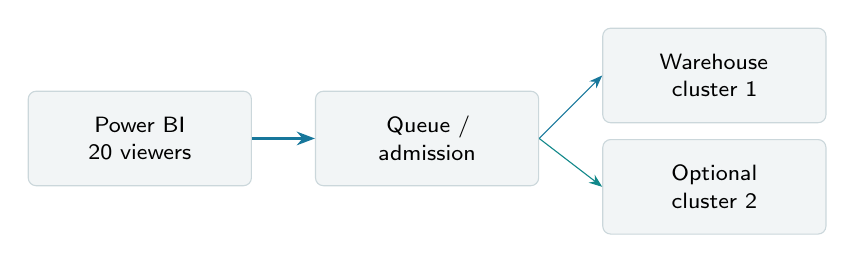
\begin{tikzpicture}[>=Stealth,every node/.style={font=\sffamily\fontsize{8}{10}\selectfont},n/.style={draw=thinrule,rounded corners=1mm,fill=papergray,align=center,text width=26mm,minimum height=12mm}]
\node[n](a){Power BI\\20 viewers};\node[n,right=8mm of a](b){Queue /\\admission};\node[n,right=8mm of b,yshift=8mm](c){Warehouse\\cluster 1};\node[n,below=2mm of c](d){Optional\\cluster 2};
\draw[->,thick,steelblue](a)--(b);\draw[->,steelblue](b.east)--(c.west);\draw[->,teal](b.east)--(d.west);
\end{tikzpicture}\\{\fontsize{8}{9}\selectfont\color{inkgray}Figure 12.3. Scaling concurrent admission is different from shortening one scan.}\end{center}
\textbf{Failure case.} A BI dashboard uses seven visuals, each generating SQL. Fifty active users can create a much more demanding query rate than fifty visual pages alone imply. Measure realistic interaction sequences and cache behaviour. \textbf{Check.} Why might an extra cluster reduce queue wait without changing the profile of an individual aggregation?
\newpage
% PAGE 218
\topic{12.4.3}{Cost-normalised capacity planning}
A good capacity study includes both \emph{latency distribution} and \emph{credits over the observation window}. For a workload with $N$ completed requests, record throughput as $N/T$ and compute spend as $C/N$ credits per successful request. If requests have different complexity, report each family separately; otherwise a changing mixture can falsely suggest a platform regression.

Snowflake's warehouse metering is not identical to per-query cost attribution. Credits billed during idle time, warehouse provisioning, shared concurrency and optional services complicate simple allocation. If you use query-level attributed compute, state exactly which Account Usage view was queried, its data latency and which cost classes are excluded. Do not infer full invoice totals from elapsed seconds alone.
\begin{whitebox}\textbf{Example (fully hypothetical, not measured)}\par
At the same workload mix, configuration A serves 100 successful requests in ten minutes at 0.20 credits for the measured interval, while B serves 160 at 0.36 credits. A: 0.002 credits/request; B: 0.00225. B offers higher throughput at a higher average credit cost per request. The choice depends on p95 target and capacity need, not a simplistic winner label.\end{whitebox}
A disciplined load test increases concurrency in stages, randomises query order, keeps a consistent data snapshot and monitors queueing as well as execution. Do not conduct a load test on a shared production warehouse without operational approval. Add auto-suspend and a spending cap in a dedicated experiment plan.
\begin{center}\renewcommand{\arraystretch}{1.08}\begin{tabularx}{\linewidth}{@{}p{31mm}XX@{}}\toprule
\textbf{Metric}&\textbf{What it says}&\textbf{What it cannot prove}\\\midrule
p95 wall time&User-facing tail&Which phase is slow\\
Execution time&Snowflake work duration&External report/render time\\
Queued overload&Capacity contention&That query SQL is inefficient\\
Credits/request&Normalised spend&Full cost without idle/services\\\bottomrule\end{tabularx}\end{center}
\repo{P137: warehouse and SQL tuning reference}{https://github.com/subhamay-bhattacharyya/snowflake-de-query-optimization}
\textbf{Check.} What workload characteristic must stay stable when comparing credits per query?
\newpage
% PAGE 219
\section*{12.5\quad Caching behavior and materialized results}
\topic{12.5.1}{Result cache and warehouse-local cache}
Snowflake can reuse a persisted query result when eligibility conditions are satisfied. The warehouse also has a local data cache that may accelerate reads after earlier scans. These are different mechanisms with different conditions, and neither is equivalent to a precomputed business mart. A query returning an already cached result can appear exceptionally fast while revealing almost nothing about the original scan's cost.
\topic{12.5.2}{Controlled warm/cold experiments}
For a baseline scan study, explicitly record whether \texttt{USE\_CACHED\_RESULT} is enabled and repeat measurements with the same policy. Even when persisted-result reuse is disabled, warehouse-local cache, data state and concurrency may vary. A ``cold run'' after resume and a ``warm run'' should be labelled operational scenarios, not interchangeable treatments. Alternate baseline and candidate query order to limit drift and do not throw away an inconvenient slow run without a documented reason.
\begin{lstlisting}[language=SQL,caption={An isolated, reversible experimental session.}]
ALTER SESSION SET USE_CACHED_RESULT=FALSE;
SELECT technology, SUM(energy_mwh)
FROM BOOK_DEV.CH12_LAB.ENERGY_FACT
GROUP BY technology;
ALTER SESSION UNSET USE_CACHED_RESULT;
\end{lstlisting}
\topic{12.5.3}{Materialization versus recomputation}
A materialised result is a design choice: precompute when the same expensive transformation is repeatedly requested, and when refresh semantics and maintenance spending are justified. Options include a scheduled Gold table, a materialized view where SQL/function restrictions allow, or a Dynamic Table with supported refresh behavior. Unlike a cached query result, these objects may incur ongoing refresh costs and operational ownership obligations.
\begin{insight}\textbf{Do not cache a semantic error.}\par
Preaggregating twelve raw revisions into a fast BI mart can make a wrong number arrive sooner. Materialization must occur after the revision-resolution and grain checks established in earlier chapters.\end{insight}
The six-row one-interval fixture is intentionally too small to motivate materialized infrastructure by runtime alone. Its purpose is to teach a correct baseline and illustrate reproducible control variables.
\repo{P013: pandas on Snowflake teaching reference}{https://github.com/Snowflake-Labs/sfguide-getting-started-with-pandas-on-snowflake}
\textbf{Check.} How would you distinguish an improved cached-result hit rate from a more selective scan?
\newpage
% PAGE 220
\section*{12.6\quad Query acceleration and search optimization concepts}
\topic{12.6.1}{Query acceleration options}
The Query Acceleration Service can provide additional compute for eligible portions of queries under supported configurations. It is not a generic speed switch for every SQL statement: eligibility, estimated benefit and consumption must be investigated. If it is activated, record service-specific credits separately from virtual-warehouse spend. A query with no qualifying work may see little improvement. The account's current feature availability, privileges and pricing must be checked before making claims in a production design.
\topic{12.6.2}{Search optimization and suitable predicates}
Search Optimization Service targets particular selective access patterns, including applicable point lookup and other documented predicates on large datasets. It maintains a search access path, which introduces maintenance and storage-related costs. It is inappropriate to enable solely because a report feels slow; first verify a suitable predicate, cardinality, data size and measured profile. For the small energy teaching fixture, ordinary range filtering is the correct starting point.
\topic{12.6.3}{Edition, cost, and support checks}
Feature support can depend on edition, object type, SQL shape, region and product evolution. A design document must state prerequisites, estimated recurring cost, pilot success metric, rollback step and service ownership. When availability is unknown, label the option a \emph{candidate for evaluation}, not an active control.
\begin{center}\renewcommand{\arraystretch}{1.08}\begin{tabularx}{\linewidth}{@{}p{31mm}XX@{}}\toprule
\textbf{Mechanism}&\textbf{Workload clue}&\textbf{Trade-off}\\\midrule
Query acceleration&Eligible costly query portions&Additional service credits\\
Search optimisation&Selective point-like access&Access-path maintenance\\
Clustering&Repeated range filtering&Background reclustering cost\\
Larger warehouse&Memory-bound heavy compute&Higher running rate\\\bottomrule\end{tabularx}\end{center}
\begin{whitebox}\textbf{Approval gate.}\par
Never enable a paid optimisation feature in the companion lab without explicit approval, a bounded pilot window and a method for verifying \emph{both} query results and metered credits. The printed code only describes read-only diagnostic queries.\end{whitebox}
\repo{P138: alternate query-performance diagnostic reference}{https://github.com/sfc-gh-hbarile/query_performance_deep_dive}
\textbf{Check.} Why should an optimisation feature's maintenance or service credits enter the final benchmark even if the query latency improves?
\newpage
% PAGE 221
\section*{12.7\quad Improving joins, filters, and aggregations}
\topic{12.7.1}{Join cardinality and filter pushdown}
The fastest fix is sometimes to remove work that never should have existed. Confirm the relationship and grain of every join. A many-to-many lookup can multiply energy rows and misstate totals; an accidental Cartesian join can create very large intermediates and spill. Push selective constraints toward inputs where doing so preserves semantics, and inspect operator cardinalities in Query Profile rather than assuming the optimiser behaves like handwritten execution order.
\topic{12.7.2}{Aggregation and column selection}
Return only columns a consumer needs; avoid \texttt{SELECT *} on wide facts when a report uses four measures. Aggregate at the approved grain rather than repeating a costly row-level join for every visual. However, an early aggregation is not safe if it discards keys needed for correct joins, changes distinctness or merges time zones incorrectly. \emph{Performance and semantics are coupled}. 
\topic{12.7.3}{Rewriting without changing semantics}
\begin{lstlisting}[language=SQL,caption={A safe baseline aggregation for the sample fixture.}]
SELECT technology, SUM(energy_mwh) AS mwh
FROM BOOK_DEV.CH12_LAB.ENERGY_FACT
WHERE interval_utc >= '2026-10-01'::TIMESTAMP_NTZ
  AND interval_utc <  '2026-10-08'::TIMESTAMP_NTZ
GROUP BY technology ORDER BY technology;
\end{lstlisting}
For the seven-day fixture, expect each technology's single-day energy multiplied by seven: Bioenergy 56, Hydro 126, Nuclear 112, Other 28, Solar 42, Wind 98, total \textbf{462.000~MWh}. The example is deliberately arithmetic, not a query-speed benchmark. Test key uniqueness after any additional dimension joins.
\begin{insight}\textbf{Rewrite review: change one idea.}\par
Do not simultaneously change warehouse size, clustering, SQL predicates and table layout. First establish exact output equivalence; then compare the targeted physical operator. If the profile does not move, reject the hypothesis and select a new one.\end{insight}
\repo{P139: Snowflake CTE Analyzer code utility}{https://github.com/dataengineerankur/SnowflakeCTEAnalyzer}
\textbf{Check.} Why can removing a duplicate join improve both latency and data quality?
\newpage
% PAGE 222
\section*{12.8\quad Benchmarking performance, credits, and latency}
\topic{12.8.1}{Workload definition and dataset snapshots}
A reproducible benchmark is a \emph{workload contract}. Specify the dataset build and immutable snapshot, schemas and row counts, query families, parameters, selectivity, arrival distributions and concurrency. Pin the warehouse and session settings, compiler-relevant SQL, benchmark window, permissions and product version where visible. A script that runs a single small \texttt{SELECT} five times is a useful teaching exercise but not a production workload assessment.

Our companion includes three query families: \textbf{daily interval selection}, \textbf{per-technology total} and \textbf{fact-to-dimension lookup}. The fixture starts with the six accepted observations from prior chapters and expands them deterministically to seven dates: \textbf{42 rows / 462.000~MWh}. The input data are synthetic and extremely small; Snowflake performance on them will be dominated by overhead, caching and environment effects. Any benchmark report must say so near its headline.
\begin{center}\renewcommand{\arraystretch}{1.1}\begin{tabularx}{\linewidth}{@{}p{35mm}XX@{}}\toprule
\textbf{Recorded field}&\textbf{Purpose}&\textbf{Sample value}\\\midrule
Input release&Same rows in every variant&synthetic-v1\\
SQL version&Comparable query semantics&baseline / candidate\\
Warehouse&Controlled compute&approved test WH\\
Cache flag&Explain reuse&persisted result off\\
Concurrency&Reproducible load&single session\\
Source evidence&Trace actual run&query ID and timestamp\\\bottomrule\end{tabularx}\end{center}
A production study must include representative volumes and customer-specific privacy constraints. Generating millions of synthetic rows may itself consume substantial credits; plan dataset build and cleanup separately from measurements.
\repo{P140: cross-platform benchmark method reference}{https://github.com/henbh/dbx-sf-benchmark}
\textbf{Check.} Which omitted benchmark variable would make a warehouse-size comparison non-repeatable?
\newpage
% PAGE 223
\topic{12.8.2}{Median, p95, credits, and repeat counts}
Mean runtime can hide tail latency. With a sample of at least several runs per variant, report the \emph{median}, \emph{p95}, minimum/maximum and sample count. State the percentile method because small samples can give unstable p95 estimates. Pair wall-clock latency with query execution and wait times; a slow BI page may not correspond to a slow query. Collect enough runs to reveal noise, alternate treatments and report uncertainty rather than choosing the best run.

A speed ratio is $S=\mathrm{median}(t_{\mathrm{baseline}})/\mathrm{median}(t_{\mathrm{candidate}})$, provided both are evaluated on equivalent inputs and correctness is established. A cost ratio is computed over identical workloads and time windows, \emph{including} idle/overhead and any enabled paid services. An apparent improvement in one query with a maintenance-heavy clustering feature may increase total account spend.
\begin{lstlisting}[language=SQL,caption={Read-only history of approved tagged runs.}]
SELECT query_id, query_tag,
       total_elapsed_time / 1000.0 AS elapsed_s,
       execution_time / 1000.0 AS exec_s,
       queued_overload_time / 1000.0 AS queue_s
FROM SNOWFLAKE.ACCOUNT_USAGE.QUERY_HISTORY
WHERE query_tag='book_ch12_energy_benchmark_v1'
ORDER BY start_time;
\end{lstlisting}
\begin{whitebox}\textbf{Illustrative numbers, not a Snowflake run.}\par
A fabricated six-run series might yield a baseline median of roughly 1.9~s and a candidate near 1.2~s, but those values establish \emph{nothing} about this platform. The companion flags every such CSV row as \texttt{synthetic\_illustration}. Genuine results require captured query IDs, Account Usage/Snowsight evidence and billing observations.\end{whitebox}
Per-query attribution and warehouse metering answer different questions. The former may exclude idle warehouse spend; the latter must be distributed carefully under concurrent use. Label each metric's source, units, reporting lag and excluded cost classes.
\repo{P117: Snowflake Labs data-eng-bench}{https://github.com/Snowflake-Labs/data-eng-bench}
\textbf{Check.} How can a faster median coexist with a worse p95, and which number matters for an on-call dashboard SLA?
\newpage
% PAGE 224
\topic{12.8.3}{Limitations and benchmark report}
A defensible report separates \emph{measurement}, \emph{interpretation} and \emph{decision}. A measurement states the environment, version, observed numbers and query IDs. An interpretation states the most likely mechanism and alternative explanations. A decision says whether to deploy, revert or collect more data, and names the owner and rollback path.

In the accompanying report template, explicitly distinguish the reproducible \textbf{offline correctness oracle} from the \textbf{fabricated performance demonstration CSV} and \textbf{real Snowflake metrics still to be collected}. No numerical speedup, p95 or credit saving for Snowflake is claimed by this chapter. If the pilot is ever run, add actual query IDs and a timestamp before replacing the placeholders.
\begin{center}\renewcommand{\arraystretch}{1.13}\begin{tabularx}{\linewidth}{@{}p{31mm}XX@{}}\toprule
\textbf{Gate}&\textbf{Required evidence}&\textbf{Fail response}\\\midrule
Correctness&Same keyed result set&Stop experiment\\
Repeatability&Run count; stable snapshot&Collect more runs\\
Diagnosis&Scan/queue/spill change&Reject hypothesis\\
Economics&Credits and auxiliary charges&Estimate TCO again\\
Deployability&Owner, permission, rollback&Do not enable feature\\\bottomrule\end{tabularx}\end{center}
\textbf{Common bias.} Selecting only queries that benefit a proposed warehouse upgrade creates an invalid cost argument. Include ordinary report queries, expensive peak-time queries and repeated user interactions. If the dataset is small, state that warehouse provisioning and fixed overhead dominate; extrapolation to hundreds of millions of records would be misleading.
\begin{insight}\textbf{The most useful outcome may be ``do not optimise''.}\par
If p95 already meets the requirement, the warehouse is inexpensive, and the query is correct, a new maintenance-intensive feature may decrease reliability for negligible benefit. Recording a rational no-change decision is successful performance engineering.\end{insight}
\repo{P141: Snowflake FinOps optimisation example}{https://github.com/Bravarthan/snowflake-finops-optimization}
\textbf{Check.} What two facts must be established before claiming a percent reduction in Snowflake credit spending?
\newpage
% PAGE 225
\section*{12.L\quad Guided lab, chapter review, and exercises}
\topic{12.L.1}{Prerequisites, inputs, environment, permissions, and cost guardrails}
\textbf{Lab mission:} compare two semantically equivalent energy-report SQL patterns, produce a correctness certificate and prepare a measurement plan. The companion includes \texttt{benchmark\_queries.sql}, \texttt{energy\_sample.csv}, \texttt{benchmark\_results.csv}, \texttt{offline\_validate.py} and \texttt{tuning\_report.md}. The results CSV is \textbf{synthetic illustration only}: it was not extracted from any warehouse.

\textbf{Offline route (no cost):} Python~3 standard library; run the offline validator and the Python unit-test command listed in the companion README. \textbf{Cloud option (billable):} only with an approved isolated database and dedicated small test warehouse, least-privilege role, auto-suspend, verified budget and explicit cleanup plan. Never run optional DDL on a shared/production account.
\topic{12.L.2}{Step-by-step procedure and selected code}
\textbf{Step 1.} Validate six source energy values, their uniqueness and \textbf{66.000 MWh} single-day sum. \textbf{Step 2.} Expand the same six values across seven UTC dates for a \textbf{42-row / 462.000 MWh} reproducible exercise. \textbf{Step 3.} Examine two query shapes: a function-based date predicate and a half-open range; confirm their resulting aggregates agree for every requested day. \textbf{Step 4.} If authorised, capture multiple tagged Query History IDs and inspect Query Profile. \textbf{Step 5.} Record medians and p95 only from actual measurements, not from the demonstration CSV.
\begin{lstlisting}[language=SQL,caption={Sample range query from the companion: 4 October only.}]
SELECT technology, SUM(energy_mwh) AS mwh
FROM BOOK_DEV.CH12_LAB.ENERGY_FACT
WHERE interval_utc >= '2026-10-04'::TIMESTAMP_NTZ
  AND interval_utc <  '2026-10-05'::TIMESTAMP_NTZ
GROUP BY technology ORDER BY technology;
\end{lstlisting}
Expected aggregate for 4 October: \textbf{66.000~MWh}. \emph{Performance expectation: none.} The fixture has no meaningful partition-scale power to demonstrate a speed improvement; query timing is environmental.
\begin{whitebox}\textbf{Output folder}\par
Submit an oracle test log, versioned benchmark SQL, environment/privilege declaration, result rows and Query IDs (if actually measured), a comparison table and an ADR stating why a change is accepted, rejected or postponed.\end{whitebox}
\newpage
% PAGE 226
\topic{12.L.3}{Expected results, assertions, failure diagnosis, and cleanup}
Expected \emph{offline} invariants: six distinct technologies per date; exactly seven dates and 42 accepted fact rows; daily generation 66.000~MWh; total 462.000~MWh; both date-filter formulations have the same keyed output; no negative energy; and the benchmark demonstration file is explicitly marked as synthetic. Failures can reveal mistaken inclusive end boundaries, duplicated joins, unstable fixture order or incorrectly treated null values. Repair the correctness model before comparing speed.

\textbf{Cleanup.} Reset \texttt{QUERY\_TAG} and the result-cache session override. With authorised ownership only, remove lab-specific tables and suspend the isolated warehouse after capturing evidence. The companion does not automatically drop objects. Do not remove data or grants belonging to other work.
\topic{12.L.4}{Foundation exercise, practitioner exercise, and production-design decision}
\begin{enumerate}
\item \textbf{Foundation (20 points).} Explain persisted result cache versus warehouse-local cache and give two sources of apparent timing improvement that are \emph{not} SQL optimisation.
\item \textbf{Practitioner (30 points).} Design a seven-day query-equivalence test, collect sufficient tagged runs on an authorised Snowflake lab (or write \emph{not measured}), and record median, p95, partitions scanned and wait/spill indicators.
\item \textbf{Architectural decision (30 points).} A Power BI dashboard slows at peak usage. Compare query rewrite, warehouse resizing, multi-cluster, clustering and a serving mart; specify the evidence necessary to reject each option.
\item \textbf{Evidence and safety (20 points).} State account permissions, budget guardrails, data provenance, rollback, time window, reviewer and unresolved limitations.
\end{enumerate}
\textbf{Chapter review.} (1) Why must query correctness precede tuning? (2) What distinguishes provisioning from overload wait? (3) When can clustering be cost-negative? (4) Why is one benchmark run insufficient? (5) Which credits are missing from per-query execution attribution?
\begin{insight}\textbf{Chapter synthesis}\par
A credible tuning claim has three legs: \emph{an equal correct answer, a repeatable explanation of the bottleneck, and a measured overall cost}. Remove one leg and the conclusion becomes guesswork. Chapter~13 extends this discipline to governance, reliability, access and cost ownership.\end{insight}
{\fontsize{8}{10}\selectfont\color{inkgray}\textbf{Authoritative technical references (reviewed 22 Oct 2026).} Snowflake Documentation: Query History; Query Profile / Snowsight Activity; Clustering Keys; Query Acceleration Service; Search Optimization Service; Warehouse considerations; Account Usage Query Attribution. \href{https://docs.snowflake.com/en/sql-reference/account-usage/query_history}{Query History}; \href{https://docs.snowflake.com/en/user-guide/ui-snowsight-activity}{Query Profile}; \href{https://docs.snowflake.com/en/user-guide/tables-clustering-keys}{Clustering}; \href{https://docs.snowflake.com/en/user-guide/query-acceleration-service}{Acceleration}. GitHub repositories cited above are external teaching references, \emph{not} executed or licensed for republication in this chapter.\par}
\end{document}
